%%%%%%%%%%%%%%%%%%%%%%%%%%%%%%%%%%%%%%%%%
% Sullivan Business Report
% LaTeX Template
% Version 1.0 (May 5, 2022)
%
% This template originates from:
% https://www.LaTeXTemplates.com
%
% Author:
% Vel (vel@latextemplates.com)
%
% License:
% CC BY-NC-SA 4.0 (https://creativecommons.org/licenses/by-nc-sa/4.0/)
%
%%%%%%%%%%%%%%%%%%%%%%%%%%%%%%%%%%%%%%%%%

%----------------------------------------------------------------------------------------
%	CLASS, PACKAGES AND OTHER DOCUMENT CONFIGURATIONS
%----------------------------------------------------------------------------------------

\documentclass[
	a4paper, % Paper size, use either a4paper or letterpaper
	12pt, % Default font size, the template is designed to look good at 12pt so it's best not to change this
	%unnumberedsections, % Uncomment for no section numbering
]{CSSullivanBusinessReport}

\addbibresource{references.bib} % BibLaTeX bibliography file


% \usepackage{background} 
% \backgroundsetup{contents=DRAFT-2} % Set your own text 

%----------------------------------------------------------------------------------------
%	REPORT INFORMATION
%----------------------------------------------------------------------------------------

\reporttitle{POKT AI Lab} % The report title to appear on the title page and page headers, do not create manual new lines here as this will carry over to page headers

\reportsubtitle{Report II} % Report subtitle, include new lines if needed

\reportauthors{Authors:\\\smallskip  Nicolas Aguirre (nicolas@poktscan.com)\\ Ramiro Rodr\'iguez Colmeiro (ramiro@poktscan.com)\\ POKTscan Data Science Team }

\reportdate{\today} % Report date, include new lines for additional information if needed

\rightheadercontent{
\includegraphics[width=3cm]{POKT_logo.png}} % The content in the right header, you may want to add your own company logo or use your company/department name or leave this command empty for no right header content

%----------------------------------------------------------------------------------------

%\usepackage[printwatermark]{xwatermark}
%\newwatermark[allpages,color=red!30,angle=45,scale=6,xpos=-2cm,ypos=0]{DRAFT}  

\usepackage{placeins}

%%%%%%%%%%%%%%%%%%%%%%%%%
% Subplots
%%%%%%%%%%%%%%%%%%%%%%%%%
%\usepackage{subcaption}
%\usepackage[labelformat=simple]{subcaption} %Para subplots con parentesis
%\renewcommand\thesubfigure{(\alph{subfigure})}


\usepackage{amsmath,amssymb,amsfonts,amsbsy,latexsym,mathtools,bm}%,bbm} 

\usepackage[acronym,toc,nomain,nonumberlist,nogroupskip]{glossaries-extra}
\setglossarystyle{alttree} %Description tabulation
\glssetwidest{Holistic Evaluation of Language Models} % Longest acronym
\makeglossaries
\loadglsentries{acronym_def} % file.tex

%%%%%%%%%%%%%%%%%%%%%%%%%
% Espacio entre palabras: \usepackage{setspace}
%%%%%%%%%%%%%%%%%%%%%%%%%
\usepackage{setspace}
\onehalfspacing
%%%%%%%%%%%%%%%%%%%%%%%%%
% Para fracciones con slash
%%%%%%%%%%%%%%%%%%%%%%%%%
\usepackage{nicefrac, xfrac}

%Texbox
\usepackage{tcolorbox}
\usepackage{lipsum}

% Quotes
\usepackage{epigraph} 

\begin{document}

%----------------------------------------------------------------------------------------
%	TITLE PAGE
%----------------------------------------------------------------------------------------

\thispagestyle{empty} % Suppress headers and footers on this page

%\begin{fullwidth} % Use the whole page width
	\vspace*{-0.075\textheight} % Pull POKT latex template logo into the top margin
	
	\hfill
\includegraphics[width=5cm]{POKT_logo.png} % Company logo

	\vspace{0.15\textheight} % Vertical whitespace

	\parbox{0.9\textwidth}{\fontsize{50pt}{52pt}\selectfont\raggedright\textbf{\reporttitle}\par} % Report title, intentionally at less than full width for nice wrapping. Adjust the width of the \parbox and the font size as needed for your title to look good.
	
	\vspace{0.03\textheight} % Vertical whitespace
	
	{\LARGE\textit{\textbf{\reportsubtitle}}\par} % Subtitle
	
	\vfill % Vertical whitespace
	
	{\Large\reportauthors\par} % Report authors, group or department
	
	\vfill\vfill\vfill % Vertical whitespace
	
	{\large\reportdate\par} % Report date
%\end{fullwidth}

\newpage

%----------------------------------------------------------------------------------------
%	DISCLAIMER/COPYRIGHT PAGE
%----------------------------------------------------------------------------------------

\thispagestyle{empty} % Suppress headers and footers on this page

%\begin{twothirdswidth} % Content in this environment to be at two-thirds of the whole page width
	\footnotesize % Reduce font size
	
	\subsection*{Disclaimer}
	
	This work was partially founded by Pocket Scan Technologies LLC, a company operating on the Pocket Network.

	\vfill % Push the following down to the bottom of the page
	
	\subsubsection*{Changelog}
	
	\scriptsize % Reduce font size further
	
	\begin{tabular}{@{} L{0.05\linewidth} L{0.15\linewidth} L{0.6\linewidth} @{}} % Column widths specified here, change as needed for your content
		\toprule
		v1.0 & 2024-05-01 & First version.\\
		\bottomrule
	\end{tabular}
%\end{twothirdswidth}

\normalsize
\newpage

%----------------------------------------------------------------------------------------
%	TABLE OF CONTENTS
%----------------------------------------------------------------------------------------

%\begin{twothirdswidth} % Content in this environment to be at two-thirds of the whole page width
    \doublespacing
    \tableofcontents % Output the table of contents, automatically generated from the section commands used in the document
    \onehalfspacing
%\end{twothirdswidth}

\newpage

%----------------------------------------------------------------------------------------
%	SECTIONS
%----------------------------------------------------------------------------------------
\section{Progress Overview}\label{sec:a}

During the month of June, the socket achieved the following milestones:

\begin{itemize}[noitemsep]
    \item Merged issues on the Test-Bench code:
    \begin{itemize}[noitemsep]
        \item \textbf{Manager}:
            \begin{itemize}[noitemsep]
                \item Add same trigger restrictions based on blocks. \footnote{\url{https://github.com/pokt-scan/pocket-ml-testbench/pull/67}}
                \item Create logic for tokenizer signature task. \footnote{\url{https://github.com/pokt-scan/pocket-ml-testbench/pull/62}}
            \end{itemize}
        \item \textbf{Sampler}:
            \begin{itemize}[noitemsep]
                \item Create logic for tokenizer signature task. \footnote{\url{https://github.com/pokt-scan/pocket-ml-testbench/pull/57}}
                \item Fix generation\_until in LM classes. \footnote{\url{https://github.com/pokt-scan/pocket-ml-testbench/pull/78}}
            \end{itemize}
        \item \textbf{Evaluator}:
            \begin{itemize}[noitemsep]
                \item Create initial code for lmeh processing. \footnote{\url{https://github.com/pokt-scan/pocket-ml-testbench/pull/60}}
                \item Add signatures tokenizer evaluation. \footnote{\url{https://github.com/pokt-scan/pocket-ml-testbench/pull/63}}
                \item Finish code for lmeh. \footnote{\url{https://github.com/pokt-scan/pocket-ml-testbench/pull/65}}
            \end{itemize}
        \item \textbf{Sidecard}:
            \begin{itemize}[noitemsep]
                \item Added endpoint for tokenizer in llm nodes. \footnote{\url{https://github.com/pokt-scan/pocket-ml-testbench/pull/56}}                
            \end{itemize}
        \item \textbf{General}:
            \begin{itemize}[noitemsep]
                \item Modularizing the tasks to allow signatures. \footnote{\url{https://github.com/pokt-scan/pocket-ml-testbench/pull/54}}
                \item Task configs: update metrics and filters. \footnote{\url{https://github.com/pokt-scan/pocket-ml-testbench/pull/80}}
                \item Added website to show metrics. \footnote{\url{https://github.com/pokt-scan/pocket-ml-testbench/pull/81}}
                \item Full ML Test bench integration. \footnote{\url{https://github.com/pokt-scan/pocket-ml-testbench/pull/83}}            
            \end{itemize}
    \end{itemize}
\end{itemize}

In June 2024, significant progress was made on the socket, culminating in the completion of various tasks and milestones. 
Finally the different components of the \gls{MLTB}, such as the Manager, Sampler, Evaluator, and Sidecard were integrated. 
This integration culminated presenting the leaderboards on a website considering the results of the corresponding task metrics.

In the next sections of the present report the details of these developments and their implications are presented. 
These sections provide an overview of the work completed, updating components initially considered, and the progress made towards the final goal of the socket.

Furthermore, looking ahead, there are several future work ideas to consider. 
These include refining the evaluation metrics further, exploring additional benchmark for extended functionalities. 
These future initiatives aim to enhance the network capacity guided by the state-of-the-art in the field of machine learning and blockchain technology.


\begin{tcolorbox}[colback=red!5!white,colframe=red!75!black]
\textbf{Note:} This report was written \today, and the Huggingface announced an update in the \gls{HFOLML} at Jun 26, 2024. 
In comparison to the socket scope, major change are related to unimplemented tasks, new metrics, and task higly related to chat models. 
On the other hand, there are tasks that just have new configs. 
This report will not cover the new Leaderboard. 
Nevertheles, at POKTscan and PNYX, we are confident that the \gls{MLTB} is ready to be developed in order to reproduce the \textbf{old} Leaderboard. 
furthermore, we except that the \gls{MLTB} will be able in a short time to be updated to the new Leaderboard. 

Addressing evaluations of \gls{LM}, a topic that is at the forefront of knowledge, has an inherently dynamic nature. 
That is to say, the constant (and increasingly accelerated) improvement of the \gls{LM} requires the development of new evaluations that have to be constantly improved. 
What happened with the \gls{HFOLML} is just the first case Pocket Network faces when it wants to support AI in it. 
At POKTscan we alert the community about this inevitable game of cat and mouse, and we encourage everyone to join the game. 
\end{tcolorbox}
\section{Language Models Benchmarks and Leaderboards}\label{sec:b}

asdadad
\section{Pocket Machine Learning Test-Bench}\label{sec:c}

The \gls{MLTB} is an off-chain element of the Pocket Network whose objective is to provide online tracking of the \gls{ML} nodes of the network. It can also be thought as an specialized and early version of a Pocket Network \emph{Watcher}~\footnote{While this is likely to change, a watcher is described here: \url{https://github.com/pokt-network/pocket-network-protocol/blob/main/utility/README.md\#33-fisherman-protocol}}.
Initially the \gls{MLTB} will be focusing on \gls{LLM} metrics, but it is designed to be agnostic of the type of service to evaluate.

\subsection{Overview of the solution}

This first version of the \gls{MLTB} is focused on implementing the \gls{LMEH} framework, specifically to be able to reproduce the tasks used to create the \gls{HF} Open \gls{LLM} leaderboard. Recreating this leaderboard for Pocket Network's nodes is not straightforward, as there are important differences between a self-hosted or centralized \gls{LLM} service and the behavior of the nodes in the network. The measurement process should be able to handle these situations:
\begin{itemize}
    \item \textbf{Service availability}: A Pocket Node is not always available to any App in the network, the random session construction means that a given node to be tested could not be reachable at a given time. Also, a node can be down due to connection issues or being a faulty node. 
    \item \textbf{Time windows}: When an App and a node are paired, the connection only last one hour~\footnote{On Morse, where sessions are 4 blocks, each of 15 minutes.}. While this time might seem large, the fact that it is finite means that at any point the node can refuse to continue answering our queries if the time is up.
    \item \textbf{Identity/quality changes}: A node is not forced to provide a fixed model, as \gls{QoS} is expected to change over time (improve, adapt to consumers choices). This means that a node's metrics should be tracked over time and not just instantly and never repeated.
\end{itemize}

These conditions shaped the test-bench design, leading us to adopt an asynchronic approach to the problem. The solution that we are proposing is shown in figure~\ref{fig:bench_overview}, where we can see that the process is articulated using 4 different modules (shown in orange), a database for the tests data or datasets (shown in blue) and coordination services (shown in white).
\begin{figure}[H]
    \centering
    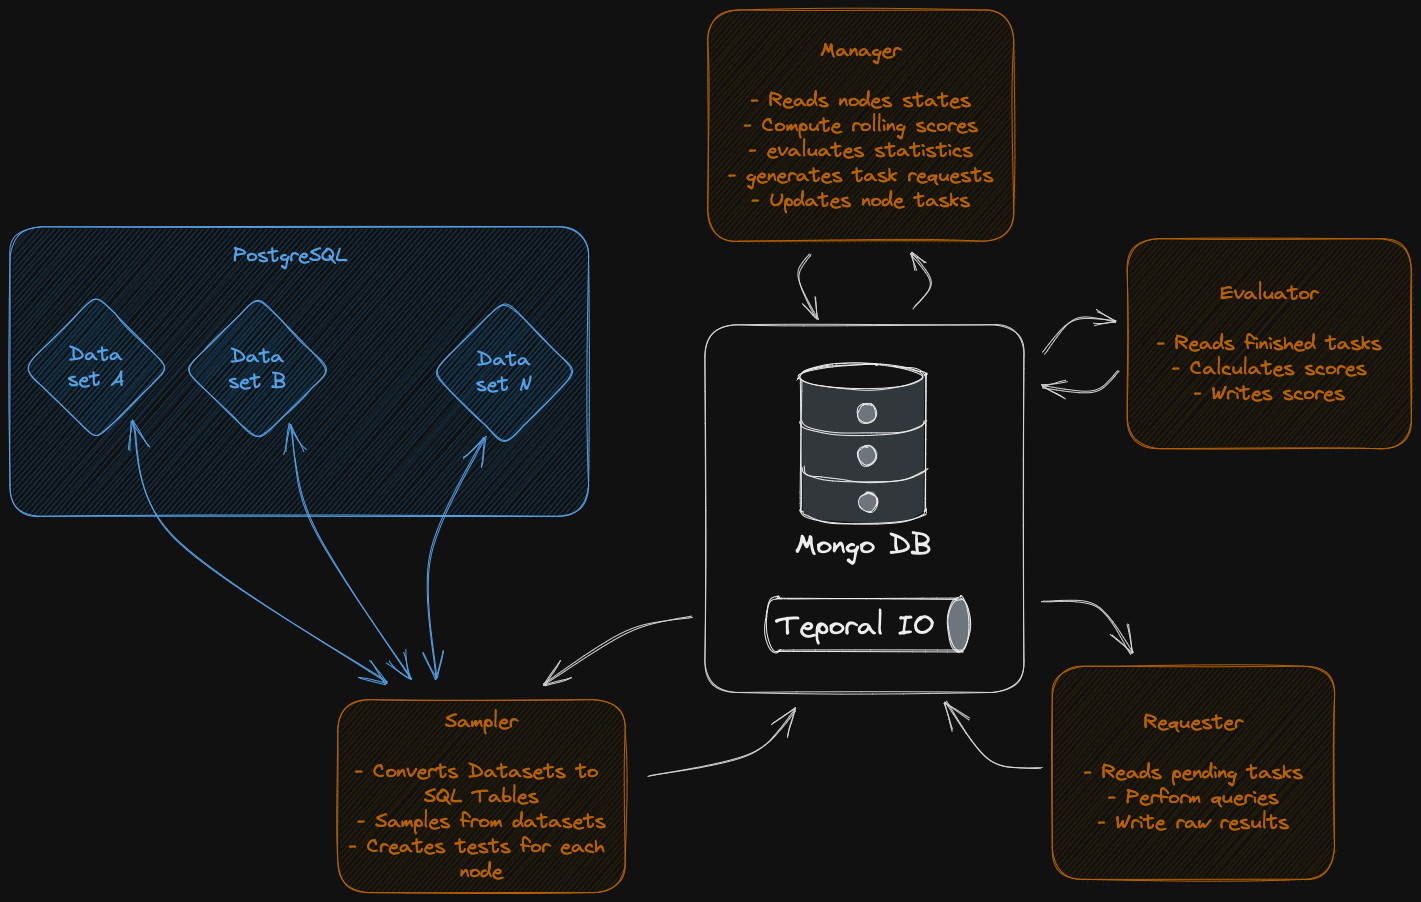
\includegraphics[width=0.95\textwidth]{bench_overview.png}
    \caption{Overview of the different elements composing the Pocket's \gls{MLTB}.}
    \label{fig:bench_overview}
\end{figure}
Each of the \gls{MLTB} four main blocks work together to track the selected \gls{CTF}s (or \emph{tasks}) scores of each of the nodes in the Pocket Network. Each of the main blocks do the following:
\begin{itemize}
    \item \textbf{Manager:} This block is in charge of keeping account of all the nodes in the networks and the scores associated with the tracked \gls{CTF}s. It will periodically refresh the list of nodes that are staked to a given Pocket Network service, review each of them and look for missing or outdated scores, remove old data, include new test results (if available from the evaluator) and request new tests (following a given strategy). Also, it is responsible of generating the average scores and other information that is later exposed to the public (i.e. generate the metrics needed to reproduce a leaderboard).
    \item \textbf{Sampler:} This block is in charge of handling the actual data that is used to generate each sample from a given \gls{CTF}. The manager gives the sampler an indication of which node to test, on which task and how many samples, with this data the sampler collects the required information and creates a generic call request for the Pocket Network. This call request is stored in a database where it waits until it can be executed. The sampler is also responsible of tracking datasets and keeping them available in a fast-access database. Each time a new \gls{CTF} is requested, a new collection will be written in the datasets database.
    \item \textbf{Requester:} All the pending requests, generated by the sampler, are consumed by this block. Its job is to interact with the Pocket Network, implementing retries, timeouts and Apps management. It controls a series of Apps that are used to make relays, it periodically checks if any of these apps is paired (in session) with a node that has pending requests and execute the requests when possible. After fulfilling a requests it writes the raw results back in the database and commands the evaluator to finish the measurement cycle. 
    \item \textbf{Evaluator:} This is the final block of the measurement process, it takes the task information and the node's response and finishes the task requirement. For each task it will create a result (a value of a metric specific to the task at hand) and write it back to the database.
\end{itemize}

The coordination of all these blocks is done using Temporal IO~\footnote{\url{https://temporal.io/}} where each block translates into a different work queues. This framework was chosen due to its robustness and scaling capabilities. As the Pocket Network grows, the number of nodes and tasks to test will grow too, in order to keep fresh track of all nodes, the measurement process needs to be easily parallelized and modular.

The data between the workers and also the data that composes the node's profiles (used to create the leaderboard) is managed using MongoDB~\footnote{\url{https://www.mongodb.com/}} because it offer us the possibility of adding new fields to the records without re-writing the whole database. This is needed when a new \gls{CTF} is added to a collection of nodes that are already in the test rotation.

To record the datasets of the different \gls{CTF} we chose to use PostgreSQL~\footnote{\url{https://www.postgresql.org/}} for ease of integration with common \gls{ML} development tools such as Torch~\cite{paszke2017automatic} and \gls{HF}.

\subsection{In-depth workings}

To keep the language concise, we opted to follow the \gls{LMEH} nomenclature to describe different parts of a \gls{CTF}. Each job in the \gls{MLTB}, an end-to-end cycle through all the apps, is a partial execution of a \gls{CTF} consisting of:
\begin{itemize}
    \item \textbf{Task:} The main element of the job, it is composed of all the information and metadata required to produce a valid Pocket Network request for a particular \gls{CTF} on a given node, including:
    \begin{itemize}
        \item Reference ID: A unique identifier of the job.
        \item Node address: Node to be tested.
        \item Service: The service that is going to be called.
        \item Evaluation: A high order grouping or framework name like \gls{LMEH} or \gls{HELM}.
        \item Task: The name of the \gls{CTF} to test, like \emph{mmlu\_high\_school\_macroeconomics}"
        \item Quantity: The amount of tests to do, a job run commonly tests only a sub-set of all the samples available in the \gls{CTF}.
        \item Blacklist: The sample indexes that should not be part of the job run. This is used to not repeat part of the \gls{CTF} on successive calls.
    \end{itemize}
    \item \textbf{Instance:} After being processed by the sampler, each task will produce an \emph{instance}. An instance is a set of calls to a Pocket Network node, it is composed of:
    \begin{itemize}
        \item Reference ID: A reference to the originating task.
        \item Node address: Node to be tested.
        \item Service: The service that is going to be called.
        \item Query list: A list of queries to perform. The length of the list will vary, as some tasks require multiple queries to the model in order to be solved. Each of the elements in this list will have all the data required to make a successful call in the Pocket Network (like \emph{method} and \emph{path} to call) and the reference IDs of the prompts.
    \end{itemize}
    \item \textbf{Prompt:} This is the actual content of the request that is going to be executed against the node. Since prompts can be lengthy, we opted for a separated collection to hold this data. Each element consists of a reference ID to the corresponding instance and the payload to be sent.
    \item \textbf{Response:} The raw result of a prompt. The outputs of the model as answer to the given prompts are stored without any change into a collection for later analysis. It also has a reference ID to the corresponding prompt.
    \item \textbf{Result:} This is the actual numerical value of a metric that was applied to a finished instance. This value is created by recovering the task metadata and performing the specific calculations over the responses. Ot is also referenced to the original task via an ID.
\end{itemize}

Each of these elements of the \gls{CTF} are in fact different collections in the Mongo database and are also the communication paths between the different blocks in the \gls{MLTB}. A closer look of the internal workings of the test-bench is presented in figure~\ref{fig:bench_detail}.
\begin{figure}[H]
    \centering
    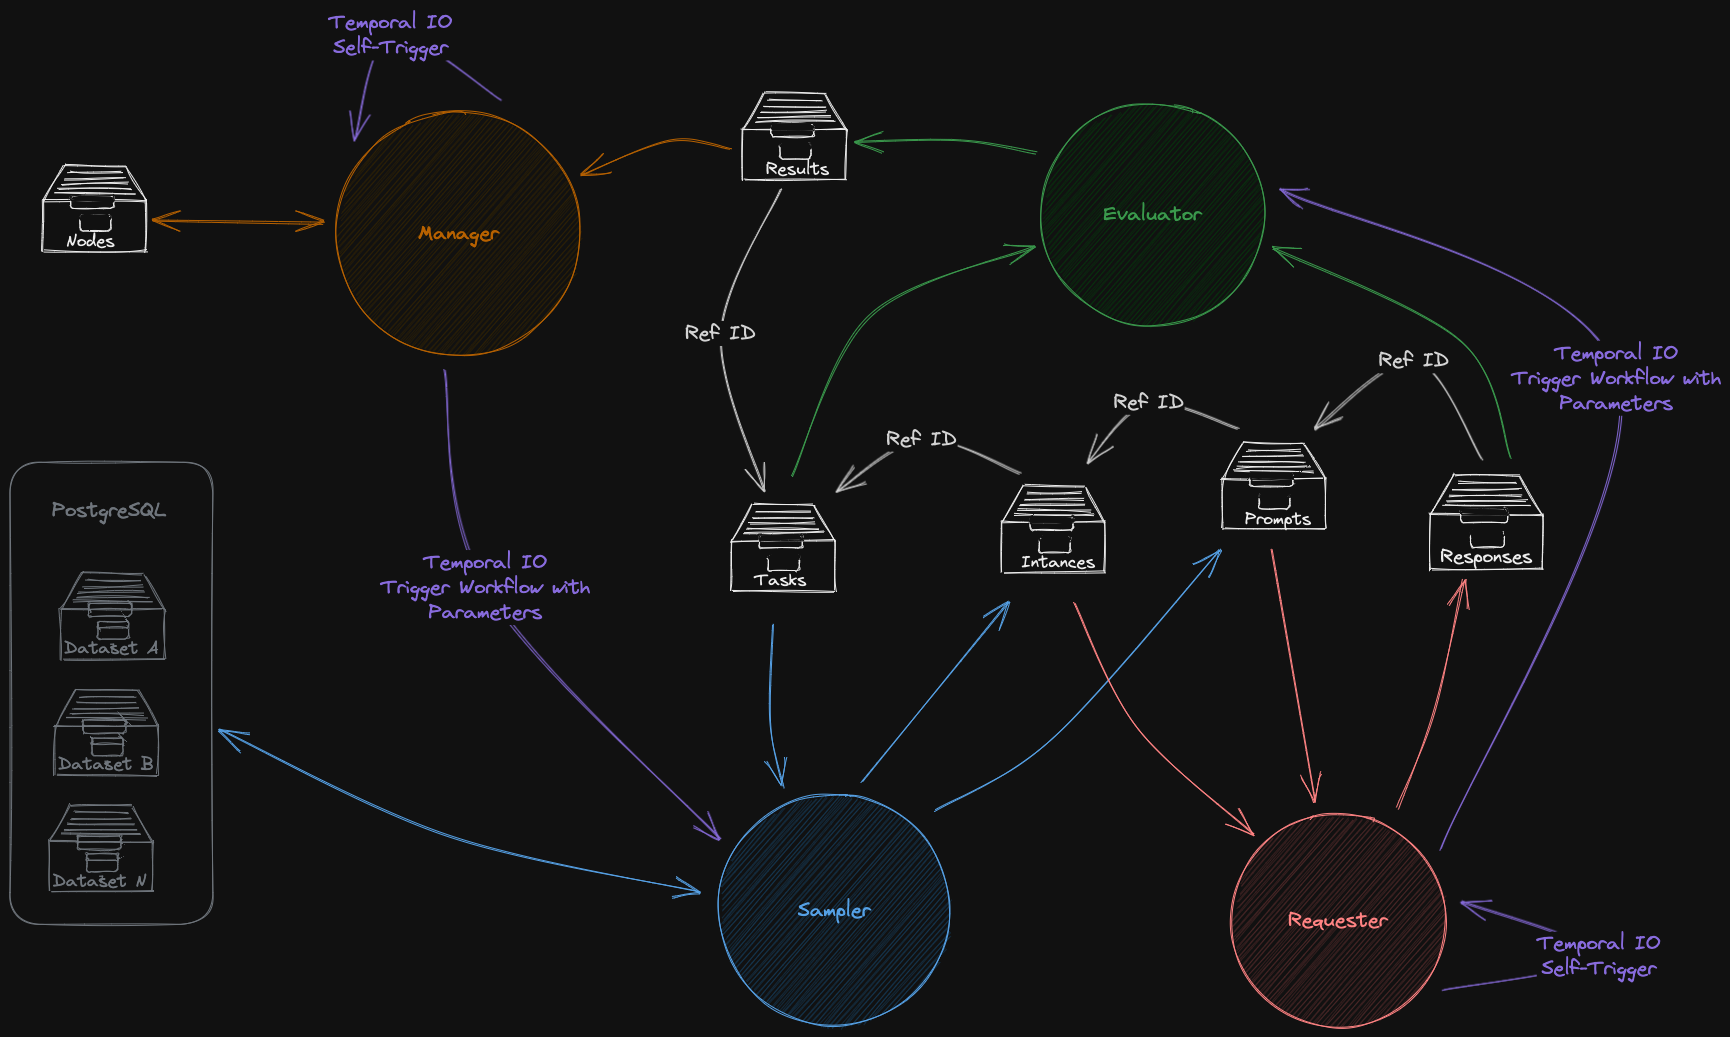
\includegraphics[width=0.95\textwidth]{bench_detail.png}
    \caption{Detail of the Pocket's \gls{MLTB} internal working, including databases relations to execution of work queues, triggering signals (in violet) and collections references for task reconstruction.}
    \label{fig:bench_detail}
\end{figure} 
The different workers' queues of the \gls{MLTB} (shown in colors: orange, blue, red and green) are controlled by the Temporal IO triggers (shown in violet). The manager and requester are the two processes controlling the workflow and executing periodically (cadency depends on configurations), they are responsible on executing the sampler and evaluator workflows respectively. The MongoDB collections are shown in white, and each collection corresponds to a part of the \gls{CTF} job being executed (described above). The PostgreSQL databases are shown in grey and they only interact with the sampler workflow.

A \gls{MLTB} job lifecicle has the following steps:
\begin{enumerate}
    \item At a given time, the manager will inspect the network nodes, find a missing task score and execute the sampler workflow with a given job config.
    \item The sampler will create a task definition and save it to the \emph{Tasks} collection, along with its instance and prompts data in their respective collections: \emph{Instances} and \emph{Prompts}. All these entries are referenced using unique job IDs. 
    \item Later, when the requester checks for sessions and finds the target node in a controlled session, it will start the prompt process. This process begins by reconstructing the prompt from the \emph{Instances} and \emph{Prompts} collections. After obtaining a response it will write it to the \emph{Responses} collections and trigger the execution of the evaluator workflow for this task.
    \item The evaluator will finally recreate the \gls{CTF} job by means of the task ID and all referencing IDs, calculate the necessary metrics and write the results in the \emph{Results} collection.
    \item The job is closed in a subsequent manager workflow execution that will read the evaluators metrics written to the \emph{Results} collection, clear the \emph{Tasks} entry (and referenced IDs) and update the \emph{Nodes} collection entry. 
\end{enumerate}


\subsection{Leaderboard Data}

The data required to recreate a leaderboard using the \gls{MLTB} data is found on the \emph{Nodes} collection. This collection has one entry per node and service~\footnote{On Shanon update there probably be a single service per node allowed, making this database have a single entry per node.} that tracks the following data:
\begin{itemize}
    \item Node address
    \item Service
    \item Last seen height (Pocket Network's block number)
    \item Last seen time (ISO date)
    \item Tasks : A vector of all the tracked \gls{CTF}s, containing:
    \begin{itemize}
        \item Evaluation : Name of the evaluation framework.
        \item Task : Name of the task or \gls{CTF}.
        \item Mean score : Mean value of the tracked scores.
        \item Std. score : Standard deviation of the tracked scores.
        \item Median score : Median value of the tracked scores.
        \item Num. samples : Number of processed samples in the configured time frame.
        \item Scores samples : Score of each of the samples tested in the configured time frame.
        \item Times : ISO date at which each of the samples was obtained.
    \end{itemize}
\end{itemize}

The collection is not created in the form of a leaderboard, it is not ordered by any kind of score, nor it calculates global scores (i.e. averages) between different tasks. However producing a replicate of any leaderboard using the provided data is trivial (its merely a grouping and averaging of tasks scores).

Its important to note that the scores calculated for each task are volatile, meaning that they are expected to change (due to normal variability in sampling strategy or node performance changes through time). They represent the instantaneous score assigned to a given task based on a number of samples that were obtained in a fixed time frame. The length of the buffer and the time frame are two configurable values that depend on different things:
\begin{enumerate}
    \item \textbf{Metric buffer length}: It determines the accuracy of the task assigned score, normally with $50$ samples it is enough to provide good approximates~\cite{polo2024tinybenchmarks}. This length also defines the time it takes the system to produce a complete run over a node, the larger the buffer, the longer it takes to be filled.
    \item \textbf{Score time frame}: Since the system is designed to evaluate models that we cannot guarantee to remain the same through time, a given time frame must be given for the samples. This time frame defines a time to live for the samples in the scores buffers, when a sample surpass this time it is erased and a process to sample a new one is created. This value is configurable, the shorter the time, the fastest the test cadence, we expect this value to be in the order of days.
\end{enumerate}
\section{Future Work}\label{sec:z}

hablar de que pokt-square no lo vamos a seguir laburando activamente.

decir cuales son las cosas que siguen en desarrollo

dar panorama para cuando primer mvp?
\newpage


%----------------------------------------------------------------------------------------
%	 Acronyms
%----------------------------------------------------------------------------------------
\printglossary[type=\acronymtype,title=List of Acronyms]

%----------------------------------------------------------------------------------------
%	 REFERENCES/BIBLIOGRAPHY
%----------------------------------------------------------------------------------------

\newpage

\addcontentsline{toc}{section}{Reference List} % Add the bibliography to the table of contents

%\begin{twothirdswidth} % Content in this environment to be at two-thirds of the whole page width
	\printbibliography[title=Reference List] % Output the bibliography with a custom section title
%\end{twothirdswidth}


%----------------------------------------------------------------------------------------

\end{document}	


